\documentclass[11pt, oneside]{amsart}
\usepackage{geometry}
\usepackage[utf8]{inputenc}
\usepackage{graphicx}
\usepackage{float}
\usepackage{etex,mathtools}
\usepackage{amssymb}
\usepackage{enumitem}
\usepackage{amsmath}
\usepackage{caption}
\usepackage{listings}
\usepackage{array}

\usepackage[colorinlistoftodos]{todonotes}

\graphicspath{{images/}}

\newif\ifnotesw \noteswtrue
\newcommand{\notes}[1]{\ifnotesw \textcolor{red}{  $\clubsuit$\ {\sf \bf \it  #1}\ $\clubsuit$ }\fi}

\title[]{Preliminary report, PGM}
\author[1]{Nicolas Jouvin}
\author[2]{Thomas Kerdreux}
\author[3]{Louis Thiry}
\begin{document}

\maketitle
\begin{abstract}
This paper presents an algorithm to learn non linear stationary dynamics of a system.
\end{abstract}

\section{The model}

%ca il faudra le placer un moment
%The system can be viewed as a graphical model :
%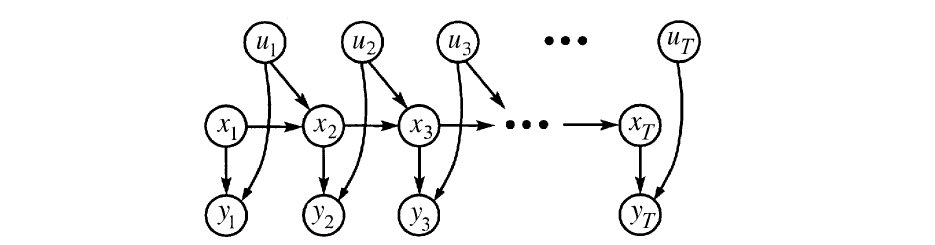
\includegraphics[width=14cm]{screenshot_graphical_model.PNG}
%\captionof{figure}{Graphical model of our system.}

We want to model a non-linear stochastic dynamics in discrete-time with the help of three sequences : $x=(x_t)_{t=1\cdots T}$, $y=(y_t)_{t=1\cdots T}$ and  $u=(u_t)_{t=1 \cdots T}$.
\begin{itemize}
  \item $u_t$ (in $\mathbb{R}^p$) are called the input variable and are observed.
  \item $x_t$ (in $\mathbb{R}^q$) are called the state and are unknown.
  \item $y_t$ (in $\mathbb{R}^n$) are called the output and are observed.
\end{itemize}


The dynamics of these data is modeled as follow:
\begin{eqnarray}
x_{t+1}&=& f(x_t,u_t)+w_t\\
y_t &=& g(x_t,u_t)+v_t
\end{eqnarray}
and can be represented with the graphical model:
\begin{figure}[H]
	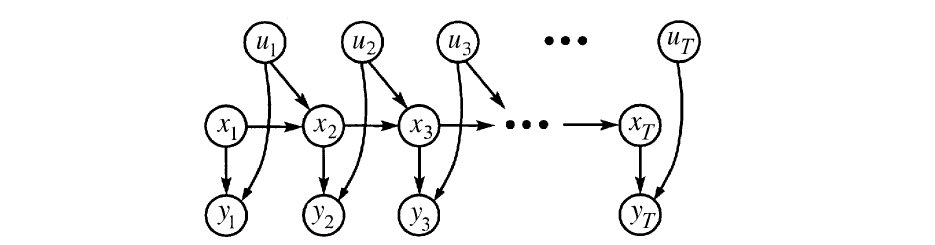
\includegraphics[width=14cm]{screenshot_graphical_model.PNG}
	\captionof{figure}{Graphical model of our system.}
\end{figure}

We see that the dynamics is therefore supposed to be Markovian, meaning a future observation depends only on the present state, and stationary because $f$ and $g$ do not depend of $t$.\\
The vector $(w_t)$ and $(v_t)$ are two \textit{i.i.d.} sequence of Gaussian random variables, with covariance matrix Q and R respectively, and represent the noise on the state space and the output. The choice of noises independant in time simply expresses the fact that, given a state $x_t$, the output $y_t$ is generated with a distribution depending only on $x_t$. 


\indent \textbf{For now $f$  and  $g$  are only assumed to be differential but otherwise arbitrary.}
Later, we will make specifical assumptions about the form of these two functions using Radial Basis Functions (RBF), allowing us to have closed form for the estimators in the \textit{M-step}, thus to compute exact M-steps.\\ 


\section{Proposed algorithm}

\textbf{Objective:}  Knowing the sequences $(y_t)_{t=1 \cdots T}$ and $(u_t)_{t=1 \cdots t}$, we want to learn the functions $f$ and $g$.
For that, we need to infer the state sequence $(x_t)_{t=1...T}$.
To achieve this, the authors propose to use an EM-algorithm.\\

%\noindent\textbf{Heuristic procedure:} The likelihood $P(Y|\text{parameters})$ appears in a non convex form because of the latent variables. To maximize it we use EM-algorithm. The procedure maximize a lower bound of the likelihood successively with respect to the parameters (f,g) (M-step) and then in respect of the latent variable (states) (E-step). The algorithm procedure is composed of three stages:\\

%\noindent\textbf{Heuristic procedure:} Call $\theta$ the parameters of our model. The likelihood $L(\theta) := P(Y, U|\theta) = \int P(Y, U, X|\theta)dX$ appears in a non convex form because of the latent variables. To maximize it we use the EM-algorithm. The procedure maximize a lower bound of the likelihood iteratively and successively. First with respect to Q a distribution on the hidden states X (E-step) and then with respect to the parameters $\theta$ of ($f$,$g$). (M-step). It is a classical result that the E-step optimum $ Q^{*}_{k+1} = P(X | Y, U, \theta^{*}_{k})$.

%This heuristic is well-known and works for a lot of problems. Now the questions are, and this is the heart of the problem : how to find an good estimate of $P(X | Y, U, \theta^{*}_{})$ and how to derive $\theta^{*}$ at each step. The authors propose a procedure for the two step which is described below :\\

\noindent\textbf{E-step:}
In the E-step, we assume that we know the functions $f$ and $g$ and we want to infer the sequence $(x_t)_{t=1...T}$.
In the case where $f$ and $g$ are linear, we can use Kalman filter to compute the conditional distributions $p(x_t|y,u)$ and then use the Rauch-Tung-Stribel smoother to estimate the conditional distributions $p(x_t|y,u)$.

Since our functions are not linear, we linearize \textbf{locally} our functions $f$ and $g$ in space around a point $\hat{x}_t$ at each step, and we can apply the filter and smoother describe below.   
\begin{align*}
	x_{t+1} &= f(\hat{x}_t, u_t) + A_{\hat{x}_t} (x - x_t) + w_t\\
	y_t &= g(\hat{x}_t, u_t) + C_{\hat{x}_t} (x - x_t) + v_t\\
\end{align*}
This approach is called the Extented Kalman Filter (EKF).\\

\noindent\textbf{M-step:}
In the M-step, we assume that we know the distributions on the states and we want to estimate the parameters of our functions $f$ and $g$.
It is a regression problem that we can't solve for differentiable arbitrary non-linear function.
Thus we restrict ourself to a specific class of non-linear functions, namely RBF functions plus an affine term. 
This specific assumption on the form of $f$ and $g$ allow the author to do parametric estimation (estimating parameters of each RBF plus the matrixes) and to derive closed form estimators. \\

\noindent\textbf{Initialization:} 
For the initialization, we need values for the parameters of the functions $f$ and $g$ to perform the Kalman filter and RTS smoother.
This initialization is a key point since the EM-algorithm leads to local maxima of the likelihood.\\

\section{Technical implementation}

As explained, the algorithm presented in this paper consist in an EM algorithm, for which we will now detail the technical aspects :
\begin{itemize}
  \item \textbf{Notations :} Since the EM algorithm consists in a loop, and that in each loop we have to run over all the state space we introduce some conventions : we will use time indices $t$ for the states ($x_t, y_t,\ldots$) and the numerical indices $k$ for the current iteration of the EM algorithm.
  
  \item \textbf{E-step.}
   As explained before, for $t \in \left [ 1; T \right ]$, we need to linearize the function $f$ and $g$ around a well chosen point $\hat{x}_t$ for both the Kalman filter and RTS smoother.
   For this, we will use for $\hat{x}_t$ the mean values of the last computed distribution. 
For the Kalman filter, we have acces to the previous smoothed conditonnal ditribution $p_{k-1}(x_t | y_1, ... , y_T)$, for each $ t \in [1, T]$, we linearize $f$ and $g$ around :
 \begin{align*}
 	\hat{x}_{t, filter} &= \mathbb{E}_{p_{k-1}}(x_t | y_1, ... , y_T)\\
\end{align*}
With these linearization, we apply the Kalman filter and we get $p_{k}(x_t | y_1, ... , y_t)$.
Then, we will re-linearize and use for $\hat{x}_t$ the mean of the filtered distributions $p_{k}(x_t | y_1, ... , y_t)$ that we  have just computed : 
 \begin{align*}
 	\hat{x}_{t, smoother} &= \mathbb{E}_{p_{k}}(x_t | y_1, ... , y_t)\\
\end{align*}
So we are able to apply an Extended Kalman Smoothing to perform the E-step and get the conditionnal probabilities on the hidden states :
    \begin{align*}
      P(x_t |u_1, ..., u_T, y_1, ... , y_T),& t \in [1,T]\\
      P(x_{t+1}, x_t |u_1, ..., u_T, y_1, ... , y_T),& t \in [1,T-1]\\
    \end{align*} 
 
  \item \textbf{M-step.}
    In the M-step, we want to learn the parameters of the functions $f$ and $g$.
    In the paper, these functions are assumed to be of the form:
    \begin{align*}
      f(x,u) &= \sum_{i=1}^I h_i \rho_i(x) + Ax + Bu + b + w\\
      \rho_i(x) &= \frac{1}{(2\pi)^{d/2}|S_i|^{1/2}} exp\left(-\frac{1}{2}(x-c_i)^TS_i^{-1}(x-c_i)\right)\\
    \end{align*}
    $w$ is a zero-mean Gaussian noise variable with covariance $Q$.
    The centers $c_i$ and width $S_i$ of the $\rho_i$ (called radial basis functions) are supposed to be known.
    With these assumptions, the value of the parameters $\theta = \left( h_1, ..., h_I, A, B, b\right)$ and $Q$ can be expressed in close form.
\item \textbf{Initilization}
We need to initialize the parameters of our RBF functions (centers $c_i$ and width $S_i$).
For that, the authors propose to run a first EM algorithm assuming that f and g are linear.
Then we place the centers of our RBF. \\
\end{itemize}




%The algorithm is first tested on generated data.
% commentaire sur la forme bien particulière de ces fonction : douille

\section{Trying to understand the M-step}
The article miss at providing a full understanding on how Radial basis functions are used to compute exactly the M-step. In order to implement safely, it is of interest to write down all the analytic computations. So let's start from the beginning:\\

At the M-step we have the knowledge of $p_{\theta_{old}}(x_k|\overline{u},\overline{y})$ and $p_{\theta_{old}}(x_k,x_{k+1}|\overline{u},\overline{y})$ for all possible value of $k$. From that we want $f$,$g$, $R$ and $Q$.\\ 

\begin{itemize}
\item The use of the EKS was in fact done in a way such that $(x_k,x_{k+1})$ are Gaussian. So the knowledge of $p_{\theta_{old}}(x_k|\overline{u},\overline{y})$ and $p_{\theta_{old}}(x_k,x_{k+1}|\overline{u},\overline{y})$ boils down to covariance matrix and mean vector. Indeed these are the output of Kallman.
\item $f$, $g$ have evolved from the land of non-linear arbitrariness to the heaven of radial basis functions. \textbf{Let's denote by $\theta_f$ and $\theta_g$, the respective parameters that stand for the representation of $f$ and $g$.}
\end{itemize}

At the M-step, we estimate the parameters $(\theta)=(\theta_f,\theta_g,R,Q)$ by maximizing L, the expected complete likelihood. To write it we use the graph factorization of $p(x,y,u)$. For any sequence $x,y,u$ we have:
\begin{eqnarray}
p_{\theta}(x,y,u)&=& p_{\theta}(x_1)\prod_{t=1}^{T-1}{p_{\theta}(x_{t+1}|x_t,u_t)}\prod_{t=1}^{T-1}{p_{\theta}(u_t)}\prod_{t=1}^{T}{p_{\theta}(y_t|x_t,u_t)}
%p_{\theta}(x,y,u)&=& p_{\theta}(x_1)\prod_{t=1}^{T-1}{\frac{p_{\theta}(x_{t+1},x_t|u_t)}{p_{\theta}(x_t|u_t)}}\prod_{t=1}^{T-1}{p_{\theta}(u_t)}\prod_{t=1}^{T}{\frac{p_{\theta}(y_t,x_t|u_t)}{p_{\theta}(x_t|u_t)}}
\end{eqnarray}
But here $y$ and $u$ are observed so that (denoting $\overline{y}$,$\overline{u}$) :
\begin{eqnarray}
%
p_{\theta}(x,\overline{y},\overline{u})&=& p_{\theta}(x_1)\prod_{t=1}^{T-1}{p_{\theta}(x_{t+1}|x_t,\overline{u}_t)}\prod_{t=1}^{T}{p_{\theta}(\overline{y}_t|x_t,\overline{u}_t)}
\end{eqnarray}

Then the expected complete likelihood (over $p_{\theta_{old}}(x_t)$ and $p_{\theta_{old}}(x_t,x_{t+1})$) is written as:
\begin{eqnarray}
L=\mathbb{E}_x(\log(p_{\theta}(x_1)))+\sum_{t=1}^{T-1}{\mathbb{E}_x(\log(p_{\theta}(x_{t+1}|x_t,\overline{u}_t)))}+\sum_{t=1}^{T}{\mathbb{E}_x(\log(p_{\theta}(\overline{y}_t|x_t,\overline{u}_t)))}\nonumber
\end{eqnarray}
\textbf{We want to maximize L and it is separable on $(\theta_f,Q)$, $(\theta_g,R)$}.\\

Section 6.2.3 explains how to maximize each $\mathbb{E}_x(\log(p_{\theta}(\overline{y}_t,x_t)))$ over $(\theta_g,R)$ (situation (3) with j=1) and $\mathbb{E}_x(\log(p_{\theta}(x_{t+1},x_t)))$ over $(\theta_f,Q)$ (situation (1) with j=1).\\
Introducing the author notations (it is the same for $g$, just replace $f$ by $g$): 
\begin{align*}
\theta_f & \overset{\Delta}{=} [h_1^f, \ldots, h_I^f, A^f, B^f, b^f] \\
\Phi_f & \overset{\Delta}{=} [\rho_1^f(x),\ldots, \rho_I^f(x), x^T, u^T, 1]^T \quad\text{(always fixed)} 
\end{align*}
we are able to obtain close form for the optimal parameters in the M-step :

\begin{eqnarray}
(\hat{\theta}_f,\hat{Q})&=&\underset{\theta_f,Q}{\text{argmin }}{\left(\sum_{t=1}^{T-1}{
<(x_{t+1}-\theta_f\Phi_f)^T Q^{-1}(x_{t+1}-\theta_f\Phi_f) >_{x_{t+1},x_t}+\log(|Q|)
}\right)}\nonumber\\
(\hat{\theta}_g,\hat{R})&=&\underset{\theta_g,R}{\text{argmin }}{\left(\sum_{t=1}^{T}{
<(y_{t}-\theta_g\Phi_g)^T R^{-1}(y_{t}-\theta_g\Phi_g) >_{y_t,x_t}+\log(|R|)
}\right)}\nonumber\\
%\hat{\pi}&=& \underset{\pi}{\text{argmax }}{\mathbb{E}_x(\log(p_{\theta}(x_1)))}\nonumber
\end{eqnarray}

Which leads to:
\begin{eqnarray}
\hat{\theta}_f&=&(\sum_{t=1}^{T-1}{<x_{t+1}\Phi_f^T >_{(x_t,x_{t+1})_{old}}})(\sum_{t=1}^{T-1}{<\Phi_f\Phi_f^T >_{(x_t,x_{t+1})_{old}}})^{-1}\\
\hat{\theta}_g&=&(\sum_{t=1}^{T}{<y_{t}\Phi_g^T >_{(x_t)_{old}}})(\sum_{t=1}^{T}{<\Phi_g\Phi_g^T >_{(x_t)_{old}}})^{-1}
\end{eqnarray}

Note that implicitly,for $f$ and $g$, $\Phi=\Phi(x_t)$.

\section{Implementation}

For now, we have implemented a linear Kalman filter and linear RTS smoother in python. 









\end{document}